% Disclosure Risk Measures for Synthetic Data - Journal of Official Statistics
% Based on SAGE LaTeX template

\documentclass[Afour,sageh,times,doublespace]{sagej}

\usepackage{moreverb,url}
\usepackage[colorlinks,bookmarksopen,bookmarksnumbered,citecolor=red,urlcolor=red]{hyperref}
\usepackage{amsmath}
\usepackage{amssymb}
\usepackage{booktabs}
\usepackage{graphicx}
\usepackage{subcaption}

\usepackage{bbm}

\newcommand{\JD}[1]{\bgroup\sffamily \color{blue} $\ll$JD : #1$\gg$\egroup}

\newcommand{\MN}[1]{\bgroup\sffamily \color{green} $\ll$MN : #1$\gg$\egroup}


\newcommand\BibTeX{{\rmfamily B\kern-.05em \textsc{i\kern-.025em b}\kern-.08em
T\kern-.1667em\lower.7ex\hbox{E}\kern-.125emX}}

\def\volumeyear{2026}

\begin{document}

\runninghead{Latner \textit{et al.}}

\title{When Privacy Measures Fail: A Theoretical Critique of Empirical Disclosure Risk Assessment for Synthetic Data}

\author{Jonathan Latner\affilnum{1}, Marcel Neunhoeffer\affilnum{1,2}, and Jörg Drechsler\affilnum{1,2,3}}

\affiliation{\affilnum{1}Institute for Employment Research, Nuremberg, Germany\\
\affilnum{2}Ludwig-Maximilians-Universität, Munich, Germany\\
\affilnum{3}University of Maryland, College Park, USA}

\corrauth{Jonathan Latner, Institute for Employment Research, Regensburger Straße 104, 90478 Nuremberg, Germany.}

\email{jonathan.latner@iab.de}

\begin{abstract}
Empirical disclosure risk measures are widely used to assess how well synthetic data protects privacy. We examine the limits of common measures, the identity disclosure measure $repU$ (replicated uniques) and the attribute disclosure measure $DiSCO$ (Disclosive in Synthetic Correct in Original), showing that they can both fail to detect known disclosure risks and may even suggest higher risks when privacy improves. Using the attacker model framework from differential privacy, we define what valid disclosure risk measures should accomplish and demonstrate that these popular measures violate these criteria under certain conditions: when synthesis retains the structure of the original data, when rare records are present, and when the attacker knows the synthesis process. Through constructed examples and real data, we highlight these failures and compare additional measures (DCAP, membership inference) within the same framework. We recommend Bayesian estimation as a standard and suggest practical strategies, including targeted review of high-risk records, hybrid screening workflows, and specific guidance for practitioners making data release decisions with existing tools.
\end{abstract}

\keywords{privacy measures, statistical disclosure control, CART, Bayesian risk estimation}

\maketitle

%%%%%%%%%%%%%%%%%%%%%%%%%%%%%%%%%%%%%%%%%%%%%%%%%%%%%%%%%%%%%%%%%%%%%%%%%%%%%%%
% SECTION 1: INTRODUCTION (DRAFTED)
%%%%%%%%%%%%%%%%%%%%%%%%%%%%%%%%%%%%%%%%%%%%%%%%%%%%%%%%%%%%%%%%%%%%%%%%%%%%%%%

\section{Introduction}

Synthetic data are now a standard approach to balancing data access and privacy protection. By generating artificial records that preserve statistical properties of confidential data without directly releasing information about real individuals, synthetic data promise to enable research and policy analysis while protecting privacy. Statistical agencies, research institutions, and private organizations increasingly turn to synthetic data as a solution for sharing sensitive information  \citep{Rubin1993, Drechsler2011, hu2024advancing,drechsler202430}. The literature generally distinguishes between partially synthetic data \citep{little1993statistical}, in which only some of the records and/or attributes are replaced by synthetic values, and fully synthetic data \citep{Rubin1993}, for which entirely new records are generated by drawing from a model fitted to the original data. While several of the early adoptions of the synthetic data approach released partially synthetic data, the recent discussions around synthetic data almost exclusively focus on fully synthetic data because of their substantially increased levels of data protection compared to partially synthetic data. Hence, we also focus only on fully synthetic data in this article and implicitly refer to full synthesis whenever we use the term synthetic data.

The appeal of synthetic data is understandable. Traditional disclosure limitation techniques, such as suppression, generalization, swapping, or noise addition, degrade data quality and can undermine analytical validity. Synthetic data, by contrast, can maintain complex statistical relationships while severing the link between released records and real individuals. Moreover, advances in machine learning have made synthetic data generation widely accessible. Numerous software packages and commercial tools now offer synthetic data generation with minimal technical expertise required \citep{Nowok2016, Ping2017}. There is a widespread perception that generating synthetic data is easy \citep{Latner2024}, and to a certain degree, this is true.

However, accessibility does not imply safety. The critical question for any synthetic data release is whether the resulting data actually protect privacy. This question has no easy answer. Unlike differential privacy, which provides formal mathematical guarantees about what can be learned from a data release, most synthetic data methods offer no such guarantees. Users must rely on empirical assessment to determine whether a synthetic dataset is safe to release.

\subsection{The Challenge of Empirical Disclosure Risk Measurement}

Empirical disclosure risk measures attempt to quantify privacy protection by examining properties of the synthetic and original data \citep{Elliot2014, Taub2018, Raab2024a}. While some argue that privacy is a property of the algorithm rather than the data \citep{Jordon2022}, empirical measures remain the primary tool available to practitioners making release decisions, and are recommended even for data generated with formal privacy guarantees \citep{Desfontaines2025}.

Given this central role, their reliability is crucial. If the measures fail to detect real risks or provide misleading signals about relative safety, empirical privacy assessment becomes unreliable.


\subsection{Our Contribution}

In this paper, we argue that commonly used empirical disclosure risk measures for synthetic data have fundamental theoretical limitations, casting their reliability into doubt. Our contribution is not merely to show that these measures can fail in specific cases, though we do demonstrate such failures, but to explain \textit{why} they fail and to identify the conceptual foundations that valid measures must possess.

We make four principal contributions.

First, we develop a conceptual framework for evaluating disclosure risk measures. Drawing on the attacker model perspective from the differential privacy literature, we argue that disclosure risk should be understood as information gain: what an attacker learns about confidential data from observing a synthetic release. We propose desiderata, i.e., formal properties that valid disclosure risk measures should satisfy, including detection of certain disclosure, monotonicity in uncertainty, and consistency with information gain. These desiderata provide criteria for evaluating any proposed measure.

Second, the most widely used disclosure risk measures were developed to assess masked or anonymized releases of original data, in which each released record corresponds to a real observation. We characterize the conditions under which these measures remain valid for synthetic data. These measures are \textit{syntactic} (they check for patterns, such as uniqueness or constant values, in the data without reference to the underlying generative process) rather than \textit{semantic} (they do not assess what an attacker can actually infer about the original data from the release). For masked original data, syntactic measures have a coherent (if imperfect) logic: a unique record can be linked to a unique individual. For synthetic data, this logic breaks down. While syntactic measures can produce misleading results in a variety of settings, the failures become particularly systematic and predictable when three aggravating factors co-occur:
\begin{enumerate}
\item the synthesis method preserves the structure of the original data,
\item the original data contains rare or unique records, and
\item the attacker knows (or can infer) the synthesis algorithm.
\end{enumerate}
When these factors are jointly present, the rare records most in need of protection are precisely those most likely to be revealed by structure-preserving synthesis, yet syntactic measures are designed for a different threat model entirely. We emphasize that these conditions are sufficient for systematic failure, not necessary: attribute disclosure risks, for example, can arise even when not all of them are met. However, the co-occurrence of these factors creates a predictable pattern of failure that our empirical illustrations demonstrate.

Third, empirical demonstrations confirm that common measures violate the proposed desiderata. Using a constructed dataset with a known unique record, we show that a very strong attacker can identify this record with certainty from synthetic data generated by a CART-based model, yet the standard identity disclosure measure ($repU$) and attribute disclosure measure ($DiSCO$) report zero risk. We further show, using real-world data, that $DiSCO$ can indicate \textit{increased} risk when privacy protection is actually \textit{improved}, a direct violation of the monotonicity property that any valid measure should satisfy. These are not edge cases or implementation errors; they are predictable consequences of the conceptual mismatch between syntactic measures and synthetic data.

Fourth, Bayesian estimation of disclosure risk as propagated by \citet{reiter2005, reiter2005using,reiter2014}, which directly measures information gain, should serve as the conceptual reference standard against which other measures are validated. While Bayesian estimation is computationally demanding, we discuss conditions under which it is tractable and propose complementary strategies, including triangulation across measures, sensitivity analysis, and stress testing, that can improve disclosure risk assessment even in the absence of ideal measures.

The remainder of this paper is organized as follows. We first develop our conceptual framework, including the attacker model perspective with a spectrum of attacker capabilities, desiderata for valid measures, theoretical failure modes, and the distinction between syntactic and semantic approaches. We then review current empirical disclosure risk measures ($repU$, $DiSCO$, Bayesian estimation, DCAP, and membership inference) and evaluate them against the desiderata. We provide empirical illustrations using both constructed and real-world data. We discuss paths toward better measurement, including targeted Bayesian assessment based on \citet{reiter2014}, hybrid strategies, and practical recommendations. Finally, we conclude with a discussion of scope, limitations, and directions for future research.



%%%%%%%%%%%%%%%%%%%%%%%%%%%%%%%%%%%%%%%%%%%%%%%%%%%%%%%%%%%%%%%%%%%%%%%%%%%%%%%
% SECTION 2: CONCEPTUAL FRAMEWORK (DRAFTED)
%%%%%%%%%%%%%%%%%%%%%%%%%%%%%%%%%%%%%%%%%%%%%%%%%%%%%%%%%%%%%%%%%%%%%%%%%%%%%%%

\section{Conceptual Framework: What Should Disclosure Risk Measures Measure?}
\label{sec:framework}

We develop a conceptual framework grounded in the attacker model perspective, articulate the types of disclosure risk that concern data custodians, and propose desiderata that valid disclosure risk measures should satisfy.

\subsection{The Attacker Model Perspective}

Disclosure risk assessment can be framed as a game between two parties. On one side, there is a statistical agency that holds confidential data and wishes to release information, preferably in a privacy-preserving way, to enable research and policy analysis. On the other side, there is an attacker who seeks to learn something from the release that they did not know previously. The fundamental question is: what can an attacker learn from a released synthetic dataset about an individual whose information they do not already possess?

This framing, which we term the \textit{attacker model perspective}, is popular in the differential privacy literature \citep{Dwork2006} but applies broadly to any privacy-preserving data release. The key insight is that disclosure risk should be understood as \textit{information gain}: the difference between what an attacker knew before observing the released data and what they know afterward.

Formally, let $D$ denote the original confidential dataset, $Z$ denote the released synthetic dataset, and $S$ denote the synthesis algorithm used to generate $Z$ from $D$. An attacker begins with prior beliefs about the contents of $D$, denoted $p(D)$. After observing $Z$, the attacker updates their beliefs to form a posterior distribution $p(D|Z, S)$. Disclosure occurs when the posterior differs substantially from the prior, that is, when the attacker has \textit{learned} something about the original data from the synthetic release.

The use of information gain as the conceptual basis for disclosure risk has been debated. \citet{Hotz2022} argue that \textit{absolute} disclosure risk, i.e., the posterior probability that an attacker can identify or attribute information to an individual, is the quantity individuals should care about, and that the prior-to-posterior comparison underlying information gain is impractical because the prior is unknowable. In response, \citet{Jarmin2023} propose a set of desiderata for disclosure risk assessment methods and evaluate three major frameworks: absolute disclosure risk, prior-to-posterior comparisons, and counterfactual comparisons (as used in differential privacy). They conclude that the prior-to-posterior and counterfactual frameworks satisfy the most desiderata, while absolute disclosure risk satisfies the fewest. Our paper complements this debate in two ways. First, while \citet{Hotz2022} and \citet{Jarmin2023} focus on the conceptual foundations and the Census Bureau's adoption of differential privacy, we focus on evaluating the specific empirical measures that practitioners use to empirically assess synthetic data, showing that $repU$ and $DiSCO$ fail even on their own terms. Second, we agree with \citet{Jarmin2023} that a desiderata-based evaluation is the right approach, and our desiderata (D1--D5) are complementary to theirs, tailored to the specific context of synthetic data disclosure risk. We also note that the strong-attacker convention \citep{reiter2014}, in which the attacker knows all records except one, substantially reduces the practical difficulty of the prior specification that \citet{Hotz2022} raises, since the prior reduces to the conditional distribution of a single record given the rest of the data.

This perspective has several important implications. First, disclosure is not a property of the synthetic data alone, but of the relationship between the synthetic data, the original data, and the attacker's background knowledge. Second, the attacker's strength matters. We consider a spectrum of attacker capabilities:

%Following the convention in the differential privacy literature, we consider a \textit{strong attacker} who knows the synthesis algorithm $S$ and has access to all records in the original data except one. This represents a worst-case scenario that provides an upper bound on disclosure risk. Third, and most critically, disclosure risk measures should quantify information gain rather than merely detect patterns in the data.

\begin{enumerate}
\item \textbf{Strong attacker:} Knows the synthesis algorithm $S$ (including hyperparameters) and has access to all records in $D$ except one. This follows the convention in the differential privacy literature \citep{Dwork2006} and provides a worst-case upper bound on disclosure risk.
\item \textbf{Intermediate attacker:} Knows the class of synthesis method (e.g., ``CART via Synthpop'') but not the exact hyperparameters; has access to some but not all original records.
\item \textbf{Weak attacker:} Knows only that the data are synthetic; has external auxiliary information but no direct access to the original data or synthesis method.
\end{enumerate}

Our empirical demonstrations use the strong attacker, which is standard for worst-case analysis. The measure failures we identify are properties of the \textit{measures}, not the attacker model: $repU$ checks uniqueness, and $DiSCO$ checks target constancy regardless of the attacker's strength. What depends on the attacker's strength is the \textit{empirical significance} of failures: absolute risk may be lower under weaker attackers, but the measures' inability to detect information-gain-based disclosure persists. 

\subsection{Types of Disclosure Risk}

The literature distinguishes several types of disclosure risk. \textbf{Identity disclosure} occurs when an attacker determines that a specific individual is present in the original dataset by linking external knowledge (quasi-identifiers) to a record. \textbf{Attribute disclosure} occurs when an attacker learns a previously unknown characteristic of an individual, given knowledge of identifying ``keys'' and seeking to infer a sensitive ``target.'' \textbf{Membership inference}, studied extensively in machine learning \citep{Shokri2017, Hayes2019, Stadler2022}, seeks to determine whether a specific individual's data was used for synthesis, a task closely related to identity disclosure but focused on dataset membership rather than record linkage. From the attacker model perspective, all types represent instances of information gain; the distinctions lie in what information the attacker begins with and what they seek to learn.

\subsection{Desiderata for Valid Disclosure Risk Measures}

From an attacker model perspective, we propose five desiderata that follow from conceptualizing disclosure risk as information gain. These are minimal validity requirements, not a wish list tailored to any particular measure.

\textbf{D1: Detection.} If an attacker can identify a record or attribute with certainty, the measure should indicate maximum risk \citep{DuncanLambert1986, DuncanLambert1989}. Formally, if $p(Y_i = c | Z, D_{-i}, S) = 1$, the measure should equal its maximum value. This is the most basic requirement: a measure that fails to detect certain disclosure is not fit for purpose.

\textbf{D2: Monotonicity in uncertainty.} Increasing the uncertainty in the synthetic data should not increase measured risk. This is analogous to the post-processing property of differential privacy \citep{Dwork2006}. Formally, if $Z'$ is a version of $Z$ with additional random perturbation, then $\text{Risk}(Z') \leq \text{Risk}(Z)$.

\textbf{D3: Monotonicity in information gain.} Risk should be monotonically related to information gain: greater information gain from the synthetic data release implies greater measured risk. Formally, if observing $Z$ shifts the attacker's posterior $p(Y_i | Z, K, S)$ further from the prior $p(Y_i | K, S)$ in scenario A than in scenario B (where the scenarios may differ in attacker knowledge $K$, synthetic data $Z$, or both), then $\text{Risk}(A) \geq \text{Risk}(B)$. This desideratum requires that the measure track what the attacker \textit{learns} from the release, not merely patterns in the synthetic data or assumptions about the attacker's strength. A measure that detects patterns unrelated to information gain, or that moves in the wrong direction relative to what an attacker actually learns, violates D3 \citep{DuncanLambert1989}.

\textbf{D4: Consistency with information gain.} Risk should reflect what an attacker \textit{learns}, not merely patterns in the data. Two synthetic datasets with identical patterns may pose different disclosure risks depending on the original data and synthesis process \citep{DuncanLambert1986, reiter2014}.

\textbf{D5: No false reassurance.} The measure should not indicate low risk when high risk exists. Understating risk is more harmful than overstating it, because the former leads to inadequate protection \citep{Elliot2014, Wagner2018}.

D1 is a special, testable instance of D5: D1 requires that certain disclosure yield maximum measured risk, while D5 is the broader principle that any material understatement is problematic. We retain both because D1 provides a sharp, falsifiable test through counterexamples, whereas D5 requires comparison to a ground truth that may not always be available.

Note that D1 is not circular with respect to Bayesian estimation: it requires only that a measure detect \textit{certain} disclosure, a minimal requirement that any reasonable measure, regardless of its computational approach, should satisfy. D4 is the most demanding desideratum, and in principle any measure that quantifies the difference between posterior and prior beliefs (whether computed via Bayes' theorem, simulation, or other means) would satisfy it. The framework does not require a Bayesian implementation; it only requires that the measure capture what an attacker learns. Alternative desiderata such as computational tractability or interpretability concern \textit{usability}, not \textit{validity}. Tractability and interpretability are valuable properties, but they do not substitute for validity. A measure that violates any of them has a fundamental theoretical limitation regardless of its practical convenience.

\subsection{Syntactic Versus Semantic Privacy Measures}

The distinction between syntactic and semantic privacy measures explains why existing disclosure risk measures fail to satisfy the desiderata. We argue that syntactic measures have \textit{conditional validity}: they provide reliable signals under some conditions but fail systematically under others.

\subsubsection{Conditional Validity of Syntactic Measures}

\textbf{Syntactic measures} assess privacy by checking for patterns in the data, such as $k$-anonymity \citep{Sweeney2002} or $\ell$-diversity \citep{Machanavajjhala2007}. For masked original data, where each released record corresponds to a real individual, these measures have a coherent logic: a unique record can be linked to a unique individual.

For synthetic data, this logic breaks down. Synthetic records do not correspond to real individuals, so the uniqueness of a synthetic record does not imply re-identification risk. Conversely, the absence of unique records does not imply protection, since an attacker who knows the synthesis algorithm can infer the original records from non-unique synthetic outputs. The fundamental issue is that syntactic measures treat synthetic data as if it were masked original data, asking ``what patterns could allow re-identification?'' rather than the correct question: ``what can an attacker learn about the original data given knowledge of the synthesis process?''

\subsubsection{Semantic Measures}

\textbf{Semantic measures} directly quantify what an attacker can learn. The Bayesian disclosure risk measure \citep{reiter2014} computes $p(Y_i | Z, D_{-i}, S)$, the posterior probability of an unknown record given the synthetic data, remaining original data, and synthesis algorithm. If the posterior equals the prior, no disclosure occurred; if it concentrates on the true value, disclosure has occurred. The disadvantages are twofold. First, the computational cost: enumerating possible record values and integrating over synthesis outcomes becomes intractable for high-dimensional data. Second, the specification of the prior $p(Y_i | D_{-i}, S)$ poses a substantive challenge: the choice of prior affects the posterior and, in turn, the measured risk, and there is no consensus on what constitutes an appropriate prior for disclosure risk assessment. This challenge is analogous to the key-specification problem for syntactic measures, though the Bayesian framework makes the assumption explicit. 

\subsection{Theoretical Failure Modes}
\label{sec:failure}

The desiderata predict three failure modes for syntactic measures.

\subsubsection{Failure Mode 1: False Negatives (Missing True Disclosure)}
\label{sec:failure:false_negatives}

A syntactic measure reports low or zero risk despite actual disclosure, violating D1 and D5. We predict this will occur when structure-preserving synthesis reveals original records through the data-generating mechanism rather than through matching uniqueness patterns.

\subsubsection{Failure Mode 2: Inverse Sensitivity (Indicating Risk When Safety Increases)}
\label{sec:failure:inverse_sensitivity}

The paradox: a measure indicates \textit{increased} risk when privacy protection has \textit{improved}, violating D2. This occurs for measures that equate ``no variation in target values'' with ``disclosive,'' since destroying target information produces precisely the constant-value pattern these measures flag.

\subsubsection{Failure Mode 3: Extreme Sensitivity to Analyst Assumptions}
\label{sec:failure:arbitrary}

In practice, the same dataset can appear ``safe'' or ``risky'' depending on which variables are designated as keys versus targets, even when the actual disclosure risk is unchanged \citep{Aggarwal2005, Sweeney2002}. In principle, key specifications should reflect realistic assumptions about the attacker's knowledge, and different assumptions should yield different risk estimates. The problem is not that results vary with key specification, which is expected, but rather that (a)~there is no principled way to determine the correct specification, (b)~the sensitivity is so extreme that the measures are effectively uninformative without a justified key specification, and (c)~unlike the Bayesian approach, where assumptions enter through the prior and are therefore explicit and transparent, syntactic measures hide their dependence on assumptions in the key/target designation. We note that the Bayesian approach faces an analogous challenge in prior specification, but at least makes the assumption visible and amenable to sensitivity analysis.

%%%%%%%%%%%%%%%%%%%%%%%%%%%%%%%%%%%%%%%%%%%%%%%%%%%%%%%%%%%%%%%%%%%%%%%%%%%%%%%
% SECTION 3: CURRENT MEASURES
%%%%%%%%%%%%%%%%%%%%%%%%%%%%%%%%%%%%%%%%%%%%%%%%%%%%%%%%%%%%%%%%%%%%%%%%%%%%%%%

\section{Current Empirical Disclosure Risk Measures}
\label{sec:measures}

\subsection{Identity Disclosure Risk (repU)}

Identity disclosure risk measures the ability to identify individuals in a dataset using a set of known characteristics, i.e., `keys'. The maximum number of keys is one less than the total number of variables in the data.

The following steps are used to calculate identity disclosure risk. For a given set of keys ($q$), the intruder will look for the unique records in the original data that are also unique in the synthetic data. $repU$ (replicated uniques) is the measure of identity disclosure risk and is defined by equation~\ref{eq:repU}:

\begin{equation}
repU = \frac{100}{N_d} \sum_{q} \mathbbm{1}[d_{q} = 1] \cdot \mathbbm{1}[s_{q} = 1]
\label{eq:repU}
\end{equation}

where $d_{q}$ is the count of records in the original data with the key combination corresponding to a given value of $q$, $s_{q}$ is the equivalent count for the synthetic data, and $\mathbbm{1}[\cdot]$ is the indicator function. Thus $\mathbbm{1}[d_{q} = 1]$ equals 1 if the key combination $q$ is unique in the original data (and 0 otherwise), and $\mathbbm{1}[s_{q} = 1]$ equals 1 if the same combination is unique in the synthetic data. The sum runs over all key combinations, and $N_d$ is the total number of records in the original data. The measure counts record-level key combinations that are unique in both datasets as a percentage of all original records.

\textbf{Theoretical critique.} The $repU$ measure is purely syntactic: it assumes matching uniqueness is necessary for disclosure, but an attacker who knows the synthesis algorithm may infer original records even when they are not unique in the synthetic data. Conversely, it treats all matching uniques as equally risky, ignoring that some matches may be coincidental. From the perspective of our desiderata, $repU$ violates D1 (it can miss certain disclosures), D4 (it measures pattern presence rather than information gain), and D5 (it can provide false reassurance). More broadly, \citet{Jarmin2023} note that empirical linking-based risk assessments currently lack a proof of concept and are ``frequently criticized for using simplistic\ldots linking algorithms\ldots and often significantly underestimate disclosure risk''; \citet{Rocher2019} provide empirical evidence that such approaches can underestimate reidentification success by orders of magnitude.

\subsection{Attribute Disclosure Risk (DiSCO)}

Attribute disclosure risk measures the likelihood of identifying a previously unknown characteristic of an individual. In this approach, an attacker has access to synthetic data, knows one or more identifiers in the original data (i.e., $q$ or keys, as above), and wants to infer a sensitive attribute ($t$). Attribute disclosure risk or $DiSCO$ (Disclosive in Synthetic Correct in Original) is the subset of records in the original data for which the keys ($q$) in the synthetic data are disclosive. $q$ is disclosive if all records in the synthetic data with the same $q$ have a constant target ($t$), i.e., no variation in $t$, as defined by equation~\ref{eq:disco}:

\begin{equation}
DiSCO = \frac{100}{N_d} \sum_q \sum_t d_{tq} \cdot \mathbbm{1}[p^s_{tq} = 1]
\label{eq:disco}
\end{equation}

where $p^s_{tq} = s_{tq}/s_{.q}$ is the proportion of synthetic records with key combination $q$ that have target value $t$, and $\mathbbm{1}[p^s_{tq} = 1]$ equals 1 if the target $t$ is uniquely determined by the keys $q$ in the synthetic data (i.e., all synthetic records with key combination $q$ have the same target value $t$). The term $d_{tq}$ counts original records with target $t$ and keys $q$, so the sum captures original records whose key-target combination is ``disclosive'' in the synthetic data. The result is divided by $N_d$ and multiplied by 100 to express risk as a percentage.

\textbf{Theoretical critique.} The $DiSCO$ measure conflates ``no variation in target values'' with ``disclosive.'' While this logic holds for masked original data, it fails for fully synthetic data: the constant value in synthetic data may bear no relationship to any individual's true value. More problematically, deliberately obscuring target values (e.g., replacing with a constant) \textit{increases} measured risk because more key combinations show constant targets, violating D2. The measure thus violates D1, D2, D4, and D5.

\subsection{Bayesian Estimation of Disclosure Risk}

Another way to evaluate disclosure risk is to adopt a Bayesian perspective, as suggested by \citet{reiter2014}. Essentially, the goal is to measure what an intruder with some prior distribution over potential original data sets can learn about the original data from the release of a synthetic data set. In a fully synthetic scenario, \citet{reiter2014} assume that an intruder wants to find out some or all of the values $y_i$ for one observation in the original database $D$. While \citet{reiter2014} illustrate the approach for the entire record, the framework applies equally to a single sensitive attribute. \citet{reiter2014} further assume that the intruder knows all other records in the database $D_{-i}$ and the data synthesis algorithm $S$. Given the released synthetic data set ($Z$), knowledge about the synthetic data generation process ($S$), and the prior distribution over the sample space of all possible values of $y_i$ ($p(Y_i|D_{-i}, S)$), the intruder wants to estimate the Bayesian posterior distribution for $Y_i$:

\begin{equation}
p(Y_i | Z, D_{-i}, S) \propto p(Z | Y_i, D_{-i}, S) p(Y_i | D_{-i}, S)
\end{equation}

From the posterior distribution, a variety of disclosure risk measures can be computed. For example, for a data set where all columns contain discrete values \citet{reiter2014} calculate the probability that the unknown record is one specific combination of values $c_s$ out of all $K$ possible combinations $c_K$ as their measure of disclosure risk for a vulnerable record:

\begin{equation}
\resizebox{0.9\columnwidth}{!}{$\displaystyle
p(Y_i = c_s | Z, D_{-i}, S) = \frac{p(Z | Y_i = c_s, D_{-i}, S) \, p(Y_i = c_s | D_{-i}, S)}{\sum_{k=1}^{K} p(Z | Y_i = c_k, D_{-i}, S) \, p(Y_i = c_k | D_{-i}, S)}
$}
\label{eq:bayesian}
\end{equation}

If this probability is close to the prior (e.g., a uniform prior would be $1/K$), then an attacker cannot learn much about the last record from the released synthetic data. However, if the attacker learns something about the original data from the released synthetic data, this probability will exceed the prior. In the worst case, the attacker can identify the last record with certainty when $p(Y_i = c_s | Z, D_{-i}, S) = 1$.

\textbf{Theoretical justification.} Unlike the syntactic measures discussed above, Bayesian estimation directly operationalizes the attacker model framework from our conceptual framework. It explicitly represents the attacker's prior beliefs, incorporates knowledge of the synthesis algorithm, and computes the posterior probability given the synthetic data. The difference between posterior and prior directly quantifies information gain, i.e., what the attacker has learned. This approach satisfies all five desiderata (Table~\ref{tab:desiderata}): it detects certain disclosure (D1), directly measures information gain (D4), and cannot provide false reassurance when disclosure risk exists (D5). For D2: adding noise to $Z$ makes the likelihood $p(Z | Y_i, D_{-i}, S)$ more diffuse across candidate values, reducing the posterior's concentration on the true value and thus reducing measured risk. For D3, the measure directly computes the divergence between the posterior and the prior, so, by construction, it is monotonically related to information gain --- if the attacker learns more, the posterior diverges further from the prior, and the measure reports higher risk.

However, this measure of disclosure risk is rarely used in practice because it is complicated to calculate, especially for more complex real-world datasets.

\subsection{Other Proposed Measures}
\label{sec:other_measures}

To assess whether the desiderata are biased toward any particular approach, we briefly evaluate two additional measures from the literature.

\textbf{DCAP (Differential Correct Attribution Probability).} Proposed by \citet{Taub2018}, DCAP measures the increase in an attacker's probability of correctly guessing a target value after observing synthetic data, compared to a baseline guess from the original data's marginal distribution. DCAP is closer to a semantic measure than $repU$ or $DiSCO$: it assesses inference accuracy rather than syntactic patterns. It partially satisfies D1 (denoted $\sim$ in Table~\ref{tab:desiderata}; it can detect improved attribution) and D2 (adding noise should reduce attribution accuracy). However, it is tied to a specific inference model (correct attribution) rather than computing the full posterior, so it may miss disclosures that manifest through narrowed uncertainty rather than changed point predictions. It does not satisfy D4 in general, as it measures a specific summary statistic (the attribution probability) rather than the full information gain.

\textbf{Membership Inference Attacks (MIA).} MIA metrics \citep{Shokri2017, Stadler2022} measure an attacker's ability to determine whether a specific individual was in the training data. By construction, MIA satisfies D1 for membership disclosure (if membership can be determined with certainty, the attack succeeds) and D2 (noisier data make membership harder to infer). However, MIA addresses a different threat than attribute disclosure: knowing that someone is in the dataset is distinct from learning their sensitive attributes. MIA partially satisfies D4 for its specific threat model but does not address attribute-level information gain.

Table~\ref{tab:desiderata} summarizes how all measures perform against the desiderata. The question marks for $repU$ on D2 and D3 reflect that adding uncertainty may increase or decrease uniqueness patterns unpredictably; for D3, $repU$ does not directly track information gain but rather uniqueness, which may or may not correlate with what the attacker learns. The question mark for $DiSCO$ on D3 arises for analogous reasons: target constancy is not monotonically related to information gain. The Bayesian measure satisfies all desiderata in principle, though computational constraints may limit practical applicability.

\begin{table}[h]
\footnotesize\sf\centering
\caption{Evaluation of measures against desiderata. Checkmarks indicate the property is satisfied; crosses indicate known violations; question marks indicate context-dependent or ambiguous relationships; $\sim$ indicates partial satisfaction. See text for discussion.\label{tab:desiderata}}
\resizebox{\columnwidth}{!}{%
\begin{tabular}{@{}lccccc@{}}
\toprule
Measure & D1 & D2 & D3 & D4 & D5 \\
\midrule
$repU$ & $\times$ & ? & ? & $\times$ & $\times$ \\
$DiSCO$ & $\times$ & $\times$ & ? & $\times$ & $\times$ \\
DCAP & $\sim$ & $\checkmark$ & $\sim$ & $\times$ & $\sim$ \\
MIA & $\checkmark^*$ & $\checkmark$ & $\checkmark$ & $\sim^*$ & $\sim$ \\
Bayesian & $\checkmark$ & $\checkmark$ & $\checkmark$ & $\checkmark$ & $\checkmark$ \\
\bottomrule
\multicolumn{6}{@{}l}{\scriptsize $^*$ For membership disclosure only; MIA does not address attribute disclosure.}
\end{tabular}%
}
\end{table}


We emphasize that this table presents a theoretical evaluation against formally defined properties. When the conditions for failure are absent (for example, when synthesis methods do not strongly preserve structure, or when the data contain few rare records), $repU$ and $DiSCO$ may provide useful, if imperfect, signals. The table identifies where each measure's theoretical guarantees hold or break down. \citet{Raab2024} proposes a workflow-based approach that uses these measures as components within a broader assessment strategy, which is consistent with our practical recommendations.




%%%%%%%%%%%%%%%%%%%%%%%%%%%%%%%%%%%%%%%%%%%%%%%%%%%%%%%%%%%%%%%%%%%%%%%%%%%%%%%
% SECTION 4: ILLUSTRATIVE EXAMPLES
%%%%%%%%%%%%%%%%%%%%%%%%%%%%%%%%%%%%%%%%%%%%%%%%%%%%%%%%%%%%%%%%%%%%%%%%%%%%%%%

\section{Illustrative Examples}
\label{sec:illustrations}

Having established theoretical grounds for concern about syntactic disclosure risk measures, we now provide empirical demonstrations that these predicted failures occur in practice. We use a constructed counterexample to demonstrate Failure Mode 1 (false negatives) and Failure Mode 2 (inverse sensitivity), then examine real-world data to test our claims about structure preservation and measure sensitivity.

\subsection{Constructed Counterexample: False Negatives and the DiSCO Paradox}

Following \citet{reiter2014}, we construct a minimal example with 1,000 observations and four binary variables. The first 999 records are sampled from a multinomial distribution covering 15 of 16 possible combinations; the 1,000th record is deliberately set to the remaining combination (1,1,1,1), making it unique. We generate synthetic data using CART-based synthesis via Synthpop in R with default settings.

\begin{figure}[h]
    \centering
    \caption{Comparison of original and synthetic data distributions}
    \begin{subfigure}{0.48\textwidth}
        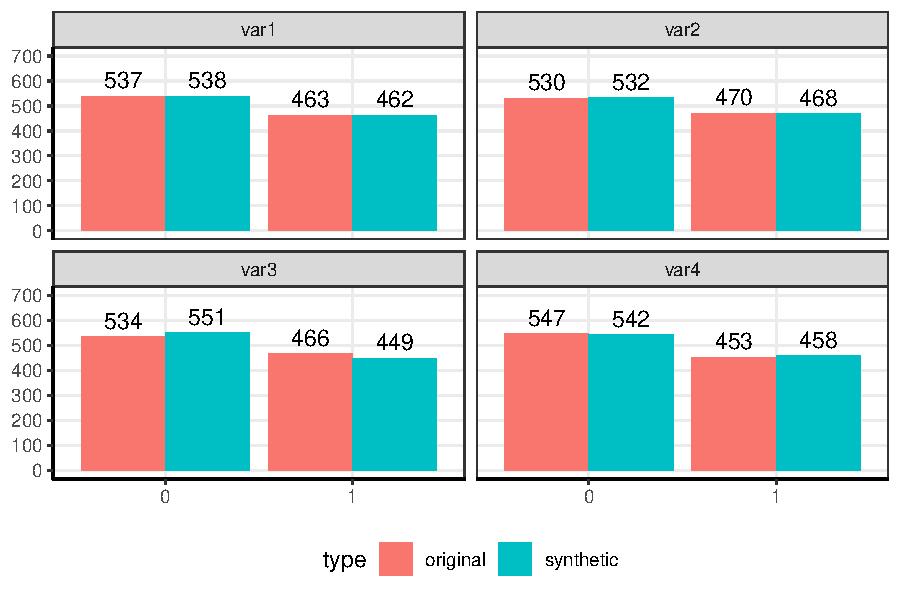
\includegraphics[width=\textwidth]{graphs/graph_cart_frequency_compare.pdf}
        \caption{Frequency distribution within variables}
        \label{fig:frequency_compare}
    \end{subfigure}
    \hfill
    \begin{subfigure}{0.48\textwidth}
        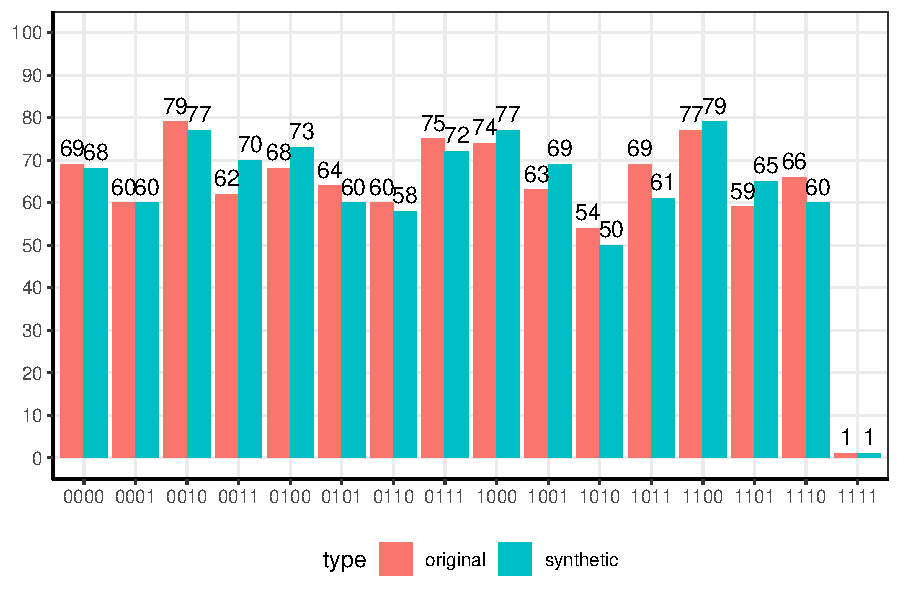
\includegraphics[width=\textwidth]{graphs/graph_cart_histogram_compare.pdf}
        \caption{Frequency histogram across all variables}
        \label{fig:histogram_compare}
    \end{subfigure}
    \label{fig:compare}
\end{figure}

Figure~\ref{fig:compare} shows that CART synthesis achieves high utility: the synthetic data closely match the original distributions. Critically, the unique record (1,1,1,1) is invisible when examining univariate distributions but reappears in the synthetic data. Across 10 synthetic datasets (Figure~\ref{fig:cart_histogram_compare_10}), the unique record reappears at least once in 8 of 10 cases.

\begin{figure*}[ht]
    \centering
    \caption{Frequency histogram: original and 10 synthetic data sets}
    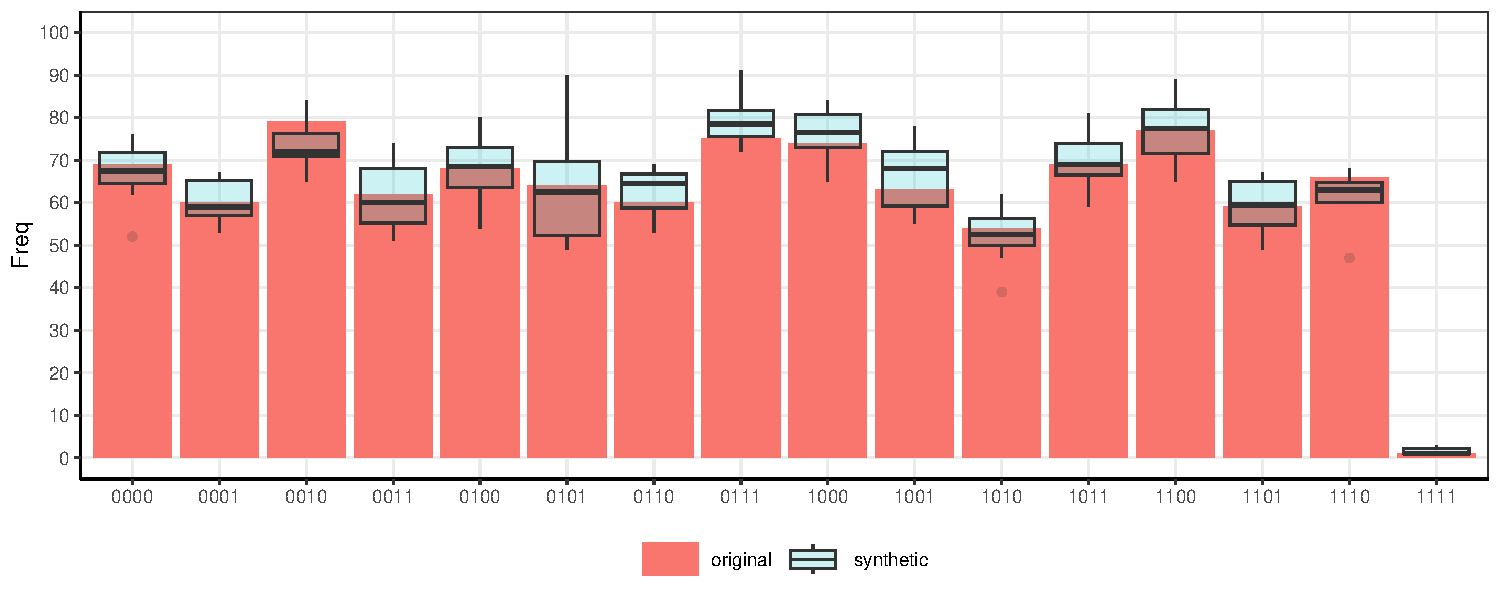
\includegraphics[width=\textwidth]{graphs/graph_cart_histogram_compare_10_v1.pdf}
    \label{fig:cart_histogram_compare_10}
\end{figure*}

\subsubsection{The Attack}

We demonstrate that an informed attacker can identify the unique record. This attack follows the framework proposed by \citet{reiter2014}, who formalize the strong attacker scenario: following their setup and the differential privacy attacker model \citep{Dwork2006}, the attacker knows the synthesis method (sequential CART) and has access to all records except the final one. They know the missing record must be one of 16 possible combinations.

The attack is straightforward: for each candidate value of the missing record, the attacker generates synthetic data and compares it to the released synthetic data. Figure~\ref{fig:attacker_default} shows the results. Only when the attacker hypothesizes that the final record is (1,1,1,1) can they reproduce synthetic data containing that combination. Conditional on observing (1,1,1,1) in the released data, the attacker knows with certainty what the final record must be.

\begin{figure*}[ht]
    \centering
    \caption{The attack: Histogram of 16 possible original datasets $\times$ 10 synthetic datasets each}
    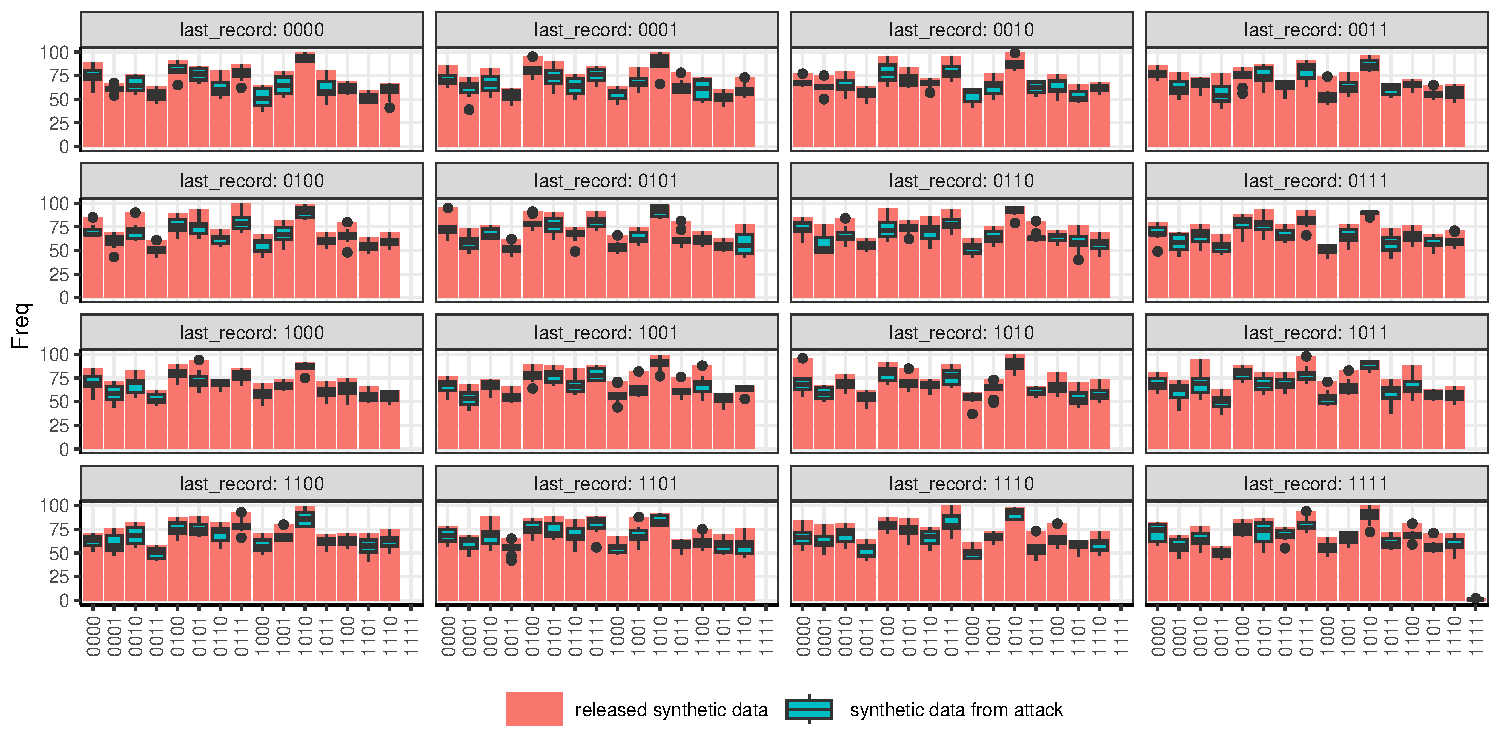
\includegraphics[width=\textwidth]{graphs/graph_attacker_default_v1.pdf}
    \label{fig:attacker_default}
\end{figure*}

\subsubsection{Measure Failure}

Table~\ref{table:disclosure_risk_1} shows disclosure risk measures for this scenario. Both $repU$ and $DiSCO$ report zero risk, despite the demonstrated disclosure. The $repU$ measure reports zero because, treating the first three variables as keys, no combination is unique in the dataset ($2^3 = 8$ possible combinations, all with multiple records). The $DiSCO$ measure reports a value of 0 because the target variable is not constant across any key combination.

\begin{table}[h]
    \centering
    \caption{Disclosure risk measures for simulated data}
    \resizebox{\columnwidth}{!}{% latex table generated in R 4.5.0 by xtable 1.8-4 package
% Fri Mar 20 10:46:09 2026
\begin{tabular}{lrrr}
  \toprule
Data & Unique & Identity Risk ($repU$) & Attribute Risk ($DiSCO$) \\ 
  \midrule
Original &   1 & 0.00 & 0.00 \\ 
  Synthetic &   1 & 0.00 & 0.00 \\ 
   \bottomrule
\end{tabular}
}
    \label{table:disclosure_risk_1}
\end{table}

In contrast, the Bayesian measure correctly identifies certain disclosure: $p(Y_i = (1,1,1,1) | Z, D_{-i}, S) = 1$ when the unique record reappears. When it does not reappear, the Bayesian measure correctly reports low risk (2--3\%; see Table~\ref{table:disclosure_risk_10} in the Appendix).

This demonstrates Failure Mode 1: syntactic measures report zero risk when disclosure is certain, violating desiderata D1 (Detection) and D5 (No false reassurance).

\subsubsection{The DiSCO Paradox: Inverse Sensitivity}

Using the same constructed data, we demonstrate Failure Mode 2. We replace the target variable (var4) with a constant value across all synthetic records, eliminating any information about individuals' true values. By construction, an attacker can learn nothing about anyone's var4.

Yet $DiSCO$ \textit{increases} from 0\% to approximately 15\%. Because the target is now constant across all key combinations, more records are flagged as ``disclosive.'' The measure indicates higher risk precisely when we have maximally protected the sensitive attribute.

This demonstrates Failure Mode 2: $DiSCO$ violates desideratum D2 (Monotonicity in uncertainty). Increasing uncertainty should not increase measured risk, yet it does. This paradox is an instance of a broader tension identified by \citet{Hotz2022}: the more accurately synthesis captures the original data, the greater the potential for disclosure, yet the syntactic measures used to assess risk are not calibrated to detect this relationship. They measure patterns in the released data rather than the information gain that accuracy enables.

\subsection{Real-World Analysis: SD2011 Data}

The constructed example demonstrates that syntactic measures can fail, even in an admittedly extreme case. But what happens with real data? We therefore conduct a series of empirical tests using real-world data from Social Diagnosis 2011 (SD2011) \citep{czapinski2011social}, included in the Synthpop package \citep{Nowok2016}. The synthpop SD2011 sample is drawn from a large-scale Polish household panel survey covering demographics, labor market activity, health, and economic conditions. It contains approximately 5,000 respondents and 35 variables of mixed types (categorical, ordinal, and semi-continuous), making it a realistic testbed for disclosure risk assessment. Following \citet{raab2026}, we generate 5 synthetic datasets using CART and examine key variables (\texttt{sex}, \texttt{age}, \texttt{region}, \texttt{placesize}) with \texttt{depress} (depression status) as the target (see Table~\ref{tab:attribute_risk_sd2011} in the Appendix for baseline attribute disclosure measures). These analyses test our theoretical claims about structure preservation (Condition A) and measure sensitivity (Failure Mode 3).

\subsubsection{Structure Preservation}
\label{sec:structure_preservation}

Our theoretical framework identifies Condition A (structure preservation) as critical: if synthesis generates only observed combinations, then observing a combination in synthetic data provides strong evidence that it existed in the original. We test how strongly this property holds in practice by identifying which key combinations in the synthetic data are \textit{novel} (never appeared in the original).

\begin{table}[h]
\footnotesize\sf\centering
\caption{Structure preservation in CART-synthesized SD2011 data.\label{tab:structure_preservation}}
\resizebox{\columnwidth}{!}{%
\begin{tabular}{@{}lrrr@{}}
\toprule
 & Original & Synthetic (avg) & \\
\midrule
Total records & 5,000 & 5,000 & \\
Unique key combinations & 3,459 & 2,936 & \\
\midrule
\multicolumn{3}{@{}l}{\textit{Novel combinations in synthetic data:}} & \\
\quad Number of novel keys & -- & 1,010 & \\
\quad Percentage of synthetic keys that are novel & -- & 34.4\% & \\
\midrule
\multicolumn{3}{@{}l}{\textit{Inference from observing a key in synthetic data:}} & \\
\quad $P(\text{key} \in D_{\text{orig}} \mid \text{key} \in D_{\text{synth}})$ & -- & 53.4\% & \\
\bottomrule
\end{tabular}%
}
\end{table}

Table~\ref{tab:structure_preservation} reveals that approximately 34\% of key combinations in CART-synthesized data are \textit{novel}. Observing a combination in synthetic data provides only modest evidence that it existed in the original: $P(\text{key} \in D_{\text{orig}} \mid \text{key} \in D_{\text{synth}}) \approx 53\%$, barely better than a coin flip.

The mechanism behind novel combinations is the sequential nature of CART synthesis. Synthpop synthesizes variables one at a time: first $v_1$, then $v_2 | v_1$, then $v_3 | v_1, v_2$, and so on. For each variable, a CART model is fit on the original data, and the synthetic value is sampled from the observed values in the terminal leaf node. Crucially, leaf nodes typically contain multiple observed values, especially for semi-continuous variables like age (which has 70+ distinct values in SD2011). When a value is sampled from a leaf, it is a valid draw given the conditioning variables, but the resulting \textit{full combination} across all key variables may never have appeared in the original data. For example, suppose the terminal node for age given sex=male and region=A contains ages $\{25, 26, 27\}$, with the original record being (male, A, 25). If the synthesizer draws age=26, the combination (male, A, 26) is novel, even though each conditional draw is valid. This effect compounds across variables: with four key variables, including age, the space of possible combinations is vast (thousands of cells), while the original data populates only a fraction of them. The result is a high rate of novel combinations whenever the joint distribution is sparse relative to the number of possible combinations.

The degree of structure preservation depends on variable cardinality, joint distribution sparsity, synthesis hyperparameters, and variable types. With low-cardinality categorical keys (as in our constructed example), structure preservation would be much stronger, and false negatives more likely.

\subsubsection{Key Sensitivity}
\label{sec:key_sensitivity}

We test Failure Mode 3 by computing $repU$ and $DiSCO$ using 98 different key specifications on the same synthetic data: all combinations of 1--4 keys drawn from seven potential key variables, with \texttt{depress} as target throughout. We expect risk to vary with key specification; the question is whether the variation is proportionate to meaningful differences in attacker knowledge or is instead driven by the measures' sensitivity to sparsity.

\begin{table}[h]
\footnotesize\sf\centering
\caption{Sensitivity of disclosure risk measures to key specification. The same synthetic data yields dramatically different risk estimates depending on which variables are designated as keys.\label{tab:key_sensitivity}}
\resizebox{\columnwidth}{!}{%
\begin{tabular}{@{}lrrrrrr@{}}
\toprule
 & \multicolumn{3}{c}{Identity Risk ($repU$)} & \multicolumn{3}{c}{Attribute Risk ($DiSCO$)} \\
\cmidrule(lr){2-4} \cmidrule(lr){5-7}
Number of keys & Min & Max & Range & Min & Max & Range \\
\midrule
1 key (n=7) & 0.0 & 1.6 & 1.6 & 0.0 & 0.3 & 0.3 \\
2 keys (n=21) & 0.0 & 6.1 & 6.1 & 0.0 & 2.7 & 2.7 \\
3 keys (n=35) & 0.0 & 12.1 & 12.1 & 0.0 & 5.4 & 5.4 \\
4 keys (n=35) & 0.2 & 14.5 & 14.3 & 0.1 & 6.7 & 6.6 \\
\midrule
Overall & 0.0 & 14.5 & 14.5 & 0.0 & 6.7 & 6.7 \\
\bottomrule
\end{tabular}%
}
\end{table}

Table~\ref{tab:key_sensitivity} reveals dramatic sensitivity. The same synthetic data yields $repU$ ranging from 0\% to 14.5\% and $DiSCO$ from 0\% to 6.7\%, depending solely on key specification. An analyst can report essentially zero risk (using \texttt{sex} alone) or substantial risk (using \texttt{age, region, placesize, edu}) for identical data.

This sensitivity is systematic: the correlation between unique key combinations and measured risk is extremely high ($r = 0.97$ for $repU$, $r = 0.92$ for $DiSCO$). The measures essentially track sparsity, which is determined almost entirely by the analyst's key specification rather than by the underlying disclosure risk. While key choices should, in principle, reflect realistic attacker knowledge, the extreme sensitivity means that, without a principled justification for one specification over another, the measures provide little guidance for release decisions. This validates Failure Mode 3: the measures' extreme sensitivity to analyst assumptions, combined with the absence of a principled way to set those assumptions, undermines their utility for disclosure risk assessment.

\subsubsection{Hyperparameter Effects}
\label{sec:minbucket_effect}

Can practitioners reduce structure preservation by adjusting synthesis hyperparameters? We test this using CART's \texttt{minbucket} parameter (minimum observations per terminal node), generating synthetic data with values ranging from 1 to 200.

\begin{table}[h]
\footnotesize\sf\centering
\caption{Effect of CART \texttt{minbucket} parameter on structure preservation and disclosure risk. Higher \texttt{minbucket} values reduce structure preservation (i.e., more novel combinations) and the measured disclosure risk.\label{tab:minbucket_effect}}
\resizebox{\columnwidth}{!}{%
\begin{tabular}{@{}rrrrrr@{}}
\toprule
\texttt{minbucket} & Unique Keys & Novel Keys & \% Novel & $repU$ & $DiSCO$ \\
\midrule
1 & 2,672 & 456 & 17.1 & 16.1 & 31.8 \\
5 (default) & 2,936 & 1,010 & 34.4 & 14.0 & 9.1 \\
10 & 3,057 & 1,259 & 41.2 & 13.1 & 6.9 \\
20 & 3,143 & 1,379 & 43.9 & 13.2 & 5.8 \\
50 & 3,318 & 1,669 & 50.3 & 12.7 & 5.9 \\
100 & 3,395 & 1,780 & 52.4 & 12.8 & 5.2 \\
200 & 3,555 & 2,105 & 59.2 & 11.6 & 4.7 \\
\bottomrule
\end{tabular}%
}
\end{table}

Table~\ref{tab:minbucket_effect} shows that higher \texttt{minbucket} values substantially reduce structure preservation: novel combinations rise from 17\% (\texttt{minbucket}=1) to 59\% (\texttt{minbucket}=200). Syntactic measures also decrease with higher \texttt{minbucket} ($r = -0.98$ for $repU$), but this reflects fewer unique records rather than necessarily reduced disclosure risk.

Practitioners can thus tune the level of structure preservation, but face a trade-off: higher \texttt{minbucket} reduces the ability to capture fine-grained patterns. This adjustment shifts the privacy-utility balance without eliminating the need for careful risk assessment.


%%%%%%%%%%%%%%%%%%%%%%%%%%%%%%%%%%%%%%%%%%%%%%%%%%%%%%%%%%%%%%%%%%%%%%%%%%%%%%%
% SECTION 5: TOWARD BETTER MEASUREMENT
%%%%%%%%%%%%%%%%%%%%%%%%%%%%%%%%%%%%%%%%%%%%%%%%%%%%%%%%%%%%%%%%%%%%%%%%%%%%%%%

\section{Toward Better Disclosure Risk Measurement}
\label{sec:better}

The preceding sections established that commonly used measures have well-defined validity boundaries. We now turn to constructive alternatives. We propose Bayesian estimation as a reference standard, discuss strategies for when exact computation is infeasible, and offer practical recommendations.

\subsection{Bayesian Estimation as Reference Standard}

The Bayesian approach \citep{reiter2014} directly operationalizes the attacker model perspective by computing the posterior probability of an unknown record given the synthetic data. It satisfies all five desiderata by construction (Table~\ref{tab:desiderata}). We propose it as the \textit{reference standard}: not that it must be used in every application, but that other measures should be validated against it in controlled settings before being trusted in practice.

\textbf{Computational complexity.} For $p$ categorical variables with $L$ levels each, exact computation requires $O(L^p)$ likelihood evaluations per record. Table~\ref{tab:complexity} provides rough feasibility estimates:

\begin{table}[h]
\footnotesize\sf\centering
\caption{Computational feasibility of Bayesian disclosure risk estimation.\label{tab:complexity}}
\begin{tabular}{@{}lccc@{}}
\toprule
Scenario & Candidates & MC sims & Time \\
\midrule
4 binary vars & 16 & 1,600 & ${\sim}$5 min \\
10 binary vars & 1,024 & 102K & ${\sim}$10 hrs \\
5 vars $\times$ 5 levels & 3,125 & 313K & ${\sim}$3 days \\
10 vars $\times$ 5 levels & $10^7$ & $10^9$ & Infeasible \\
\bottomrule
\end{tabular}
\end{table}

These estimates assume 100 Monte Carlo synthesis runs per candidate value, sequential CART synthesis of ${\sim}$1,000 records on a single-core consumer machine (${\sim}$3s per synthesis). Parallelization scales proportionally.

\subsection{When Exact Computation is Infeasible}

For high-dimensional real-world data, full Bayesian computation over all records is typically impractical. Three strategies can bridge the gap.

\textbf{Targeted assessment of high-risk records.} Rather than computing Bayesian risk for every record, practitioners can focus on those most likely to be vulnerable: records with unique or rare key combinations in the original data. Table~\ref{tab:sd2011_outliers} illustrates this approach for SD2011. We identified 5 records that are unique on the key variables (\texttt{sex}, \texttt{age}, \texttt{region}, \texttt{placesize}) and computed their Bayesian disclosure risk.

\begin{table}[h]
\centering
\caption{Disclosure risk for naturally occurring unique records in SD2011.
         repU and DiSCO show average values across all synthetic datasets;
         Bayesian risk shows posterior probability of correct target inference
         for each individual unique record.}
\label{tab:sd2011_outliers}
\resizebox{\columnwidth}{!}{\input{tables/table_disclosure_risk_sd2011_outliers_v2.tex}}
\end{table}

% % latex table generated in R 4.5.0 by xtable 1.8-4 package
% Fri Mar 20 10:06:03 2026
\begin{table}[ht]
\centering
\caption{Disclosure risk for naturally occurring unique records in SD2011.
             repU and DiSCO show average values across all synthetic datasets;
             Bayesian risk shows posterior probability of correct target inference
             for each individual unique record.} 
\label{tab:sd2011_outliers}
\begin{tabular}{rlccrrr}
  \toprule
Record & Key Variables & Target & In Synth & repU & DiSCO & Bayesian \\ 
  \midrule
  1 & FEMALE, 57, RLubuskie, URBAN 100,000-200,000 & 6 & Yes & 14.0 & 9.1 & 0.02 \\ 
    3 & FEMALE, 18, RMazowieckie, URBAN 500,000 AND OVER & 0 & Yes & 14.0 & 9.1 & 0.04 \\ 
    4 & FEMALE, 78, RPodlaskie, RURAL AREAS & 16 & Yes & 14.0 & 9.1 & 0.06 \\ 
    6 & MALE, 20, RSlaskie, URBAN 100,000-200,000 & 5 & Yes & 14.0 & 9.1 & 0.06 \\ 
    8 & MALE, 39, RLubuskie, URBAN 100,000-200,000 & 4 & Yes & 14.0 & 9.1 & 0.04 \\ 
   \bottomrule
\end{tabular}
\end{table}


The results are striking: syntactic measures report $repU = 14\%$ and $DiSCO = 9.1\%$ as global averages, but these figures conflate high-risk and low-risk records indiscriminately. The targeted Bayesian assessment reveals that even for these uniquely identifiable records, the posterior probability of correct inference is low (0.02--0.06), because CART synthesis introduces sufficient noise that the attacker cannot reliably reconstruct target values. This demonstrates that syntactic and semantic measures can point in opposite directions: syntactic measures flag aggregate-level patterns while Bayesian assessment reveals record-level risk.

\textbf{Approximate methods.} Monte Carlo approximation, as illustrated in our constructed counterexample, provides a general-purpose approach: simulate the synthesis process under different hypotheses about the unknown record and compare simulated outputs to the released data. Importance sampling can focus computational effort on high-probability regions of the candidate space. For synthesis methods with known analytical properties, further simplifications may be available.

\textbf{Hybrid strategies.} Syntactic measures can serve as a \textit{screening} tool within a broader assessment workflow: high syntactic risk should trigger closer investigation, but low syntactic risk should \textit{not} be taken as reassurance without further checks. Structure preservation (Table~\ref{tab:structure_preservation}) can serve as a diagnostic: when structure preservation is low, syntactic measures are less likely to miss disclosures; when it is high, semantic assessment becomes critical. This is consistent with the workflow approach advocated by \citet{Raab2024}.

\subsection{Practical Recommendations}

Based on our analysis, we offer the following recommendations for practitioners assessing the disclosure risk of synthetic data:

\begin{enumerate}
\item \textbf{Check structure preservation before interpreting syntactic measures.} Compute the overlap between original and synthetic key combinations (Table~\ref{tab:structure_preservation}). When overlap is high, syntactic measures are more likely to miss information-gain-based disclosures.
\item \textbf{Compute risk across multiple key specifications.} If risk estimates vary dramatically across plausible key sets (as in Table~\ref{tab:key_sensitivity}), this instability itself signals unreliable measurement.
\item \textbf{Target Bayesian assessment for high-risk records when feasible.} Even a small-scale assessment of unique or rare records (Table~\ref{tab:sd2011_outliers}) can reveal whether syntactic measures are providing reliable signals.
\item \textbf{Tune hyperparameters to manage structure preservation.} Higher \texttt{minbucket} values reduce structure preservation at the cost of utility (Table~\ref{tab:minbucket_effect}).
\item \textbf{Never rely on a single measure.} Triangulate across identity disclosure, attribute disclosure, and (where feasible) Bayesian measures. Consistent signals across approaches are more trustworthy than any single estimate.
\item \textbf{Document the attacker model explicitly.} Specify which attacker strength is assumed, what background knowledge is attributed, and how these assumptions affect the risk assessment.
\end{enumerate}


%%%%%%%%%%%%%%%%%%%%%%%%%%%%%%%%%%%%%%%%%%%%%%%%%%%%%%%%%%%%%%%%%%%%%%%%%%%%%%%
% SECTION 6: DISCUSSION
%%%%%%%%%%%%%%%%%%%%%%%%%%%%%%%%%%%%%%%%%%%%%%%%%%%%%%%%%%%%%%%%%%%%%%%%%%%%%%%

\section{Discussion}
\label{sec:discussion}

The validity boundaries and practical strategies in this paper suggest a path forward that preserves the usefulness of syntactic measures while acknowledging their limits. We organize the remaining discussion around practical implications, scope, limitations, and future directions.

\subsection{Practical Implications}

The persistence of syntactic measures in practice, despite their conceptual limitations, reflects a genuine tension. As \citet{raab2026} argue, $repU$ and $DiSCO$ were designed as practical tools within a specific workflow: they are intended to be used alongside other checks, with awareness of their limitations, and with the understanding that they measure specific, well-defined properties rather than providing comprehensive risk assessment. 

Our concern is that in practice, these measures are often used as standalone risk indicators to justify data releases, without the workflow safeguards their developers recommend. It is this gap between intended and actual use that motivates our formal analysis. Semantic measures, particularly Bayesian estimation, are computationally demanding and not yet ready for routine deployment in all settings. Practitioners who rely solely on syntactic measures may therefore be receiving misleading information: a measure that reports low risk may be missing real disclosures, while a measure that reports high risk may be flagging patterns that pose no actual threat. We believe practitioners should establish that they are operating within the validity boundaries of the measures before relying on them for release decisions, and that syntactic measures should be validated against semantic measures in settings similar to the intended application.

\subsection{Scope and Limitations}

Our primary attacker model assumes a strong adversary who knows the synthesis algorithm and all original records except one, providing an upper bound on disclosure risk. Our results establish that the measures \textit{can} fail, not that they \textit{always} fail.

Our empirical illustrations focused on CART-based synthesis because CART produces data with high statistical utility and, in principle, low disclosure risk \citep{Little2025, Dankar2021}. Other synthesis methods (including parametric models, GANs, and Bayesian nonparametric approaches; \citep{ManriqueVallier2018}) may exhibit varying degrees of structure preservation; extending the empirical analysis across synthesis methods is an important area for future work. However, the theoretical critique applies to any synthesis method assessed using syntactic measures: the disconnect between pattern detection and information gain is a property of the measures, not the algorithm. We did not address partially synthetic data, which warrants separate treatment.

\subsection{Future Directions}

The gap between syntactic and semantic measurement creates an opportunity for methodological innovation. Developing computationally tractable approximations to Bayesian disclosure risk estimation, whether through Monte Carlo methods, variational approximations, or exploiting structure in common synthesis methods, would address the primary barrier to the adoption of semantic measures. Equally important is a systematic empirical study of when syntactic measures provide reliable signals and when they do not: identifying the conditions under which $repU$ and $DiSCO$ approximate semantic risk would provide valuable guidance for practitioners.

Extending the framework to continuous variables and high-dimensional data would broaden its applicability, and integrating disclosure risk assessment with formal privacy guarantees, such as differential privacy, represents another promising direction. Finally, guidelines and best practices for synthetic data release should be updated to reflect the measurement limitations we have identified, so that practitioners know the limits of current measures.

A further limitation of current syntactic measures, noted by \citet{Jarmin2023} as Desideratum H (composition), is that neither $repU$ nor $DiSCO$ can accumulate disclosure risk across multiple synthetic data releases drawn from the same confidential source. Each release is assessed independently, with no framework for tracking cumulative risk. 


%%%%%%%%%%%%%%%%%%%%%%%%%%%%%%%%%%%%%%%%%%%%%%%%%%%%%%%%%%%%%%%%%%%%%%%%%%%%%%%
% ACKNOWLEDGEMENTS AND DECLARATIONS
%%%%%%%%%%%%%%%%%%%%%%%%%%%%%%%%%%%%%%%%%%%%%%%%%%%%%%%%%%%%%%%%%%%%%%%%%%%%%%%

\begin{acks}
This work was supported by a grant from the German Federal Ministry of Research, Technology, and Space (BMFTR grant number 16KISA096) with funding from the European Union NextGenerationEU. Reproducible files are located here: \url{https://github.com/jonlatner/KEM_GAN/tree/main/latner/projects/simulation}
\end{acks}

\begin{dci}
The authors have no competing interests to declare that are relevant to the content of this article.
\end{dci}


%%%%%%%%%%%%%%%%%%%%%%%%%%%%%%%%%%%%%%%%%%%%%%%%%%%%%%%%%%%%%%%%%%%%%%%%%%%%%%%
% REFERENCES
%%%%%%%%%%%%%%%%%%%%%%%%%%%%%%%%%%%%%%%%%%%%%%%%%%%%%%%%%%%%%%%%%%%%%%%%%%%%%%%

% Use SAGE Harvard bibliography style
\bibliographystyle{SageH}
\bibliography{references}


%%%%%%%%%%%%%%%%%%%%%%%%%%%%%%%%%%%%%%%%%%%%%%%%%%%%%%%%%%%%%%%%%%%%%%%%%%%%%%%
% APPENDIX
%%%%%%%%%%%%%%%%%%%%%%%%%%%%%%%%%%%%%%%%%%%%%%%%%%%%%%%%%%%%%%%%%%%%%%%%%%%%%%%
\newpage
\appendix

\section{Supplementary Tables and Figures}
\label{appendix}

\begin{table*}[ht]
    \centering
    \caption{Frequency statistics for original and 10 synthetic data sets}
    \input{tables/table_frequency.tex}
    \label{table:frequency_10_data_sets}
\end{table*}

\begin{table}[h]
    \centering
    \caption{Disclosure risk measures from 10 synthetic data sets}
    \label{tab:disclosure_risk_10}
    \resizebox{\columnwidth}{!}{% latex table generated in R 4.5.0 by xtable 1.8-4 package
% Fri Mar 20 10:46:10 2026
\begin{tabular}{lrrr}
  \toprule
Data & Unique & Identity Risk ($repU$) & Attribute Risk ($DiSCO$) \\ 
  \midrule
Original &   1 & 0.00 & 0.00 \\ 
  Synthetic 1 &   1 & 0.00 & 6.60 \\ 
  Synthetic 2 &   0 & 0.00 & 6.60 \\ 
  Synthetic 3 &   1 & 0.00 & 6.60 \\ 
  Synthetic 4 &   3 & 0.00 & 0.00 \\ 
  Synthetic 5 &   2 & 0.00 & 6.60 \\ 
  Synthetic 6 &   1 & 0.00 & 0.00 \\ 
  Synthetic 7 &   3 & 0.00 & 6.60 \\ 
  Synthetic 8 &   0 & 0.00 & 0.00 \\ 
  Synthetic 9 &   1 & 0.00 & 6.60 \\ 
  Synthetic 10 &   1 & 0.00 & 0.00 \\ 
   \midrule 
Average &  & 0.00 & 3.96 \\ 
   \bottomrule
\end{tabular}
}
    \label{table:disclosure_risk_10}
\end{table}

\begin{table}[h]
    \centering
    \caption{Attribute disclosure risk for \texttt{depress} (SD2011)}
    \resizebox{\columnwidth}{!}{\input{tables/table_disclosure_risk_sd2011.tex}}
    \label{tab:attribute_risk_sd2011}
\end{table}

\begin{figure*}[ht]
    \centering
    \caption{Compare original and synthetic data with different hyperparameters}
    \begin{subfigure}{0.48\textwidth}
        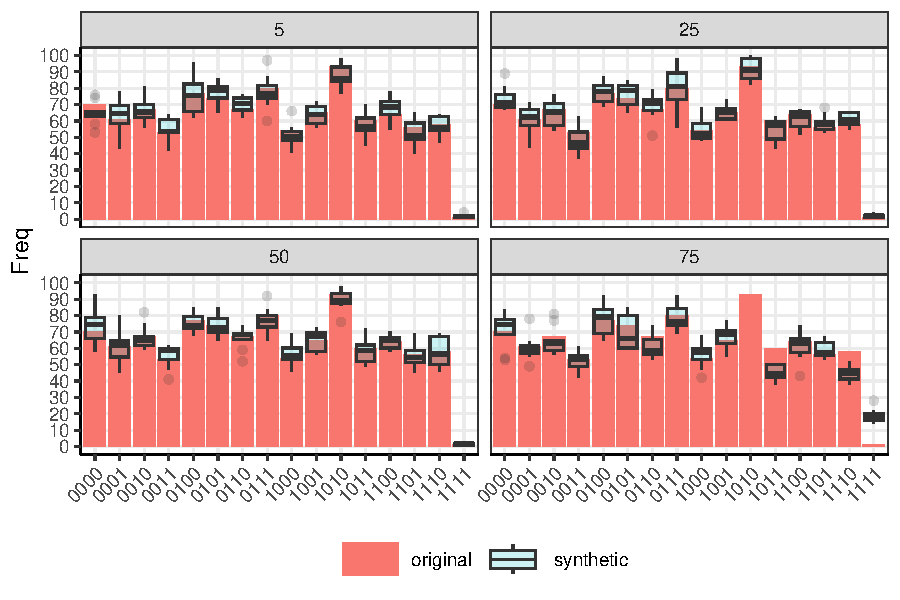
\includegraphics[width=\textwidth]{graphs/graph_cart_modified_mb_histogram_compare_10_v2.pdf}
        \caption{Minimum bucket parameter (default is 5)}
        \label{fig:attacker_modified_mb_sensitivity}
    \end{subfigure}
    \hfill
    \begin{subfigure}{0.48\textwidth}
        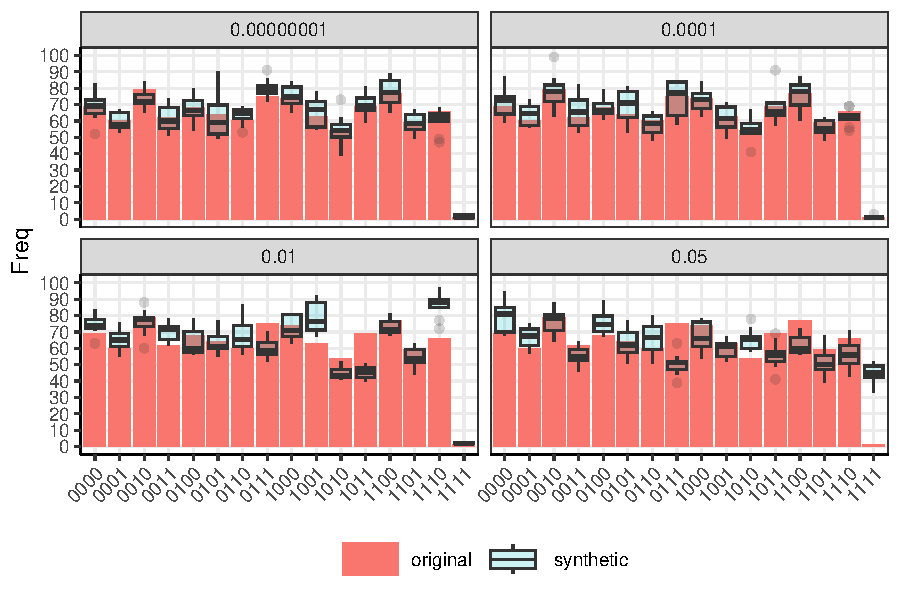
\includegraphics[width=\textwidth]{graphs/graph_cart_modified_cp_histogram_compare_10_v2.pdf}
        \caption{Complexity parameter (default is $10^{-8}$)}
        \label{fig:attacker_modified_cp_sensitivity}
    \end{subfigure}
    \label{fig:compare_modified_sensitivity}
\end{figure*}

\end{document}
